\chapter{Wolterミラー評価実験の手法に関する検討}
\thispagestyle{empty}
\label{chap3}
\graphicspath{{chap3/figure/}}
\minitoc

\newpage
%%%%%%%%%%%%%%%%%%%%%%%%%%%%%%%%%%%%%%%%%%%%%%%%%%%%%%%%%%%%%%%%%%%%%%%%%%%%%


% ================================================== %
% section
% ================================================== %
\section{諸言}
\label{chap3_introduction}

2章では、Wolterミラーの誤差応答シミュレーションを行った。
4章および5章では、
本章では、ミラーによる集光ビームを計測し\ref{chap2}章で示した各誤差要因の情報を求める上で必要となる位相回復法について、その理論を述べた上で

\clearpage
\newpage

% ================================================== %
% section
% ================================================== %

\section{位相回復法の概要}

2章でも述べた通り、波面計測は波動光学に基づいており、X線の伝播は複素波動場として与えられる。
一方で、CCDカメラなどの撮像素子で得られるのはその振幅の2乗、つまりエネルギーの情報のみである。
つまり、求めたい複素波動場に対して、カメラによる撮影では位相の情報を計測することができない。
一般にこれは位相回復問題と呼ばれ、様々な解決方法が提案されている。

いま、位相回復問題とは計測対象の画素数を縦横とも$n$として、$n \times n$の計測値を元に$n \times n$の未知数を求めることと定式化できる(図\ref{fig:phase_retrieval_problem})。
位相回復法では、どの方法においても共通の方針を取る。
未知数を求めるためには、それらを含む方程式を十分な数立てることが必要だが、一般に求める光学波動場において強度と位相の間に拘束関係はない。
そこで、焦点面に加えてもう1つ平面を定義し、その平面と焦点面の間の光学波動場の伝播を関係式として与えることで、未知数は増えるもののそれらを含む方程式を得ることができる。
これを図\ref{fig:phase_retrieval_policy}に示す。
波動場の伝播はKirhihoff-Helmholtz方程式の解として表され、距離や開口サイズに応じて近似公式が多く知られている。中でも、十分遠方においてフーリエ変換の関係で表されることが知られている。これについては、appendixにおいて詳説する。
波動場の伝播は$n \times n$の離散領域に対して$n \times n$本の数式で表される。
これだけでは未知数が$3n \times n$個に対して方程式が$n \times n$本と少なく、未知数を全て決定することができない。
そこで、未知数を減らす、もしくは関係式を増やすといった工夫を行うことで、解を決定するという方針を取る。

\begin{figure}[!ht]
\centering
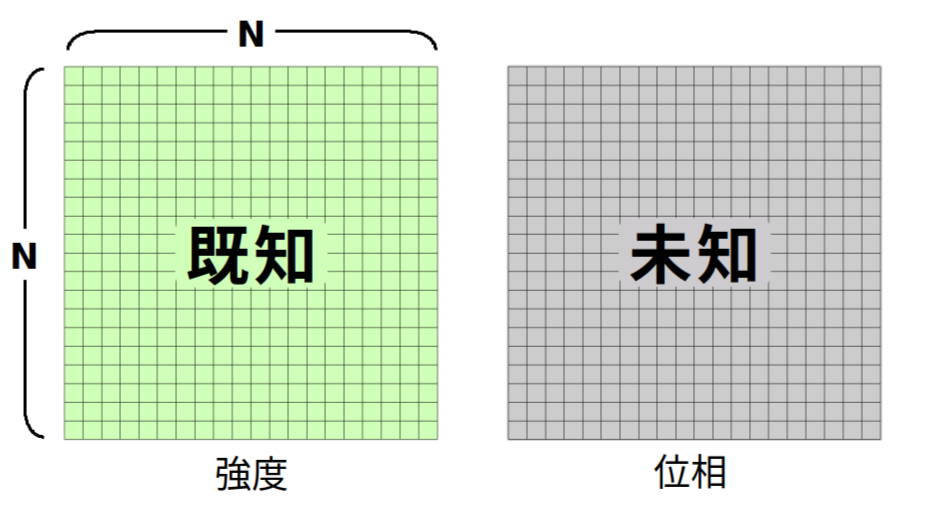
\includegraphics[width=10cm]{phase_retrieval_problem.png}
\caption{位相回復問題}
\label{fig:phase_retrieval_problem}
\end{figure}

\begin{figure}[!ht]
\centering
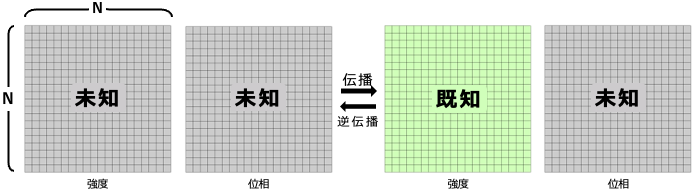
\includegraphics[width=10cm]{phase_retrieval_policy.png}
\caption{位相回復法の方針}
\label{fig:phase_retrieval_policy}
\end{figure}

以下では、代表的な解法を紹介し、続いてそれらを用いた天文用Wolterミラーの波面計測に関するシミュレーションの結果を示す。


\clearpage
% ================================================== %
% section
% ================================================== %
\newpage

\section{ダイナミックレンジ}
位相回復計算を行う上で非常に重要になるのが、カメラのダイナミックレンジである。
カメラには検出可能な強度範囲と分解能があり、検出したい波面の最大強度が範囲に収まるように取らなければならない。
最大強度が検出可能な範囲に収まるようにNDフィルターなどで光源強度を調節すると、それに応じて検出可能な最小強度が決定される。
例えば、16bitで検出可能なカメラであれば、最大強度の$\frac{1}{65535}$が検出可能な最小強度となり、これより弱い光は強度0として検出される。
このような規格化・量子化を行ったうえで回復できるかどうかを検討することが、位相回復計算の実用において不可欠である。
本研究では、Bitran社のBQ-85Mを用いて計測実験を行う。
そのパラメータを表\ref{tb:ccd_camera_params}に示す。
本章では、ダイナミックレンジを考慮しない理想の系で測定した場合、および示したカメラのダイナミックレンジにおいて測定が可能かどうかを判別する。

\begin{table}
\begin{center}
  \begin{tabular}{|c|c|l|} \hline
    項目 & 値 \\ \hline
    製品名 & BQ-85M \\
    ピクセルサイズ & 9.0 um \\
    画素 & 4096 $\times$ 4096 \\
    受光面積 & 36.8 mm $\times$ 36.8 mm \\
    A/Dコンバータ & 16bit (65535階調) \\ \hline
  \end{tabular}
  \caption{CCDカメラのパラメータ}
  \label{tb:ccd_camera_params}
\end{center}
\end{table}



\clearpage
% ================================================== %
% section
% ================================================== %
\newpage

\section{疎条件の利用}
主にCDI(コヒーレント回折イメージング)の文脈において、波動場が到達しない領域を定数0として与えることで未知数をの総数を激減させるという方法が多く取られる。
CDIとは、図\ref{fig:cdi_schematic}に示すように、サンプルに集光ビームを照射し、その回折像を見ることでそのサンプルの内部構造を解析する方法である。
位相回復法によってディテクターでの位相およびサンプル面における位相・強度を求めることで、サンプル各点における透過率を求めることが目標となる。
このような系においては、カメラの画素をより細かく取ることにより、対応するサンプル面での領域がサンプルより大きく広がるため、この領域には波面が存在しないという仮定を用いて回復計算を行うことができる。
本研究で対象とするWolterミラーについても、回復の対象である輪帯状でかつ細い波面は、下流端開口面全体に対して面積が非常に小さく、同様の方法が有効である。
CDIで広く使われているアルゴリズムの1つが、HIO(Hybrid Iterative Engine)であり、この系にも適用することが可能である。以下にその概要を示す。

\begin{figure}[!ht]
\centering
\includegraphics[width=10cm]{cdi_schematic.png}
\caption{位相回復問題}
\label{fig:cdi_schematic}
\end{figure}


\clearpage
% ================================================== %
% section
% ================================================== %
\newpage

\section{タイコグラフィ法}
前節で述べた疎条件の利用には、
前節で述べた方法について、用いるオブジェクトには大きく分けて2種類ある。1つは透過関数として表現される

\clearpage
% ================================================== %
% section
% ================================================== %
\newpage



\section{ディテクター走査による冗長性}


\clearpage
% ================================================== %
% section
% ================================================== %
\newpage

\section{下流端開口走査による冗長性}

\subsection{対称性}

\clearpage
% ================================================== %
% section
% ================================================== %
\newpage


\section{結論}
\label{chap3_conclusion}
結論を述べる。




%%%%%%%%%%%%%%%%%%%%%%%%%%%%%%%%%%%%%%%%%%%%%%%%%%%%%%%%%%%%%%%%%%%%%%%%%%%%%
%%% Local Variables:
%%% mode: katex
%%% TeX-master: "../thesis"
%%% End:
